
%(BEGIN_QUESTION)
% Copyright 2011, Tony R. Kuphaldt, released under the Creative Commons Attribution License (v 1.0)
% This means you may do almost anything with this work of mine, so long as you give me proper credit

In this process, maple syrup is heated as it passes through a steam heat exchanger, then enters an evaporator where the water boils off.  The purpose of this is to raise the sugar concentration of the syrup, making it suitable for use as a food topping.  A level control system (LT, LIR, LIC, and LV) maintains constant syrup level inside the evaporator, while an analytical control system (AT, AIR, AIC, and AV) monitors the sugar concentration of the syrup and adjusts steam flow to the heat exchanger accordingly.

$$\includegraphics[width=15.5cm]{i02934x01.eps}$$

Examine the live variable values shown in the above diagram, and then determine where any problems may exist in this syrup concentrating system. 

\vskip 20pt \vbox{\hrule \hbox{\strut \vrule{} {\bf Suggestions for Socratic discussion} \vrule} \hrule}

\begin{itemize}
\item{} A valuable principle to apply in a diagnostic scenario such as this is {\it correspondence}: identifying which variables correspond at different points within the system, and which do not.  Apply this comparative test to the variables scenario shown in the diagram, and use the results to defend your answer of where the problem is located and what type of problem it is.
\end{itemize}

\underbar{file i02934}
%(END_QUESTION)





%(BEGIN_ANSWER)

The one glaring discrepancy we see here is between the laboratory's measurement of syrup concentration and what the AIC and AIR indicate.  Given that both the AIC and AIR agree with each other on PV value, we may conclude that the signal to both of these instruments corresponds to a 34\% measurement.  The problem is either the transmitter (AT) mis-measuring the syrup concentration, or else it is sensing the concentration okay but outputting the wrong 4-20 mA signal nonetheless, or else the laboratory made a measurement error of their own and incorrectly reported a syrup concentration that is too high.

\vskip 10pt

We also see some minor discrepancies between controller output indications and actual valve stem positions, but these are small enough to ignore.  Likewise, the discrepancy between the level gauge (LG) indication and the level controller/recorder indications is small enough that it does not pose a serious problem.

%(END_ANSWER)





%(BEGIN_NOTES)


\vskip 20pt \vbox{\hrule \hbox{\strut \vrule{} {\bf Suggestions for Socratic discussion} \vrule} \hrule}

\begin{itemize}
\item{} Explain why the AIR cannot be at fault in this scenario.
\item{} Explain why the AIC cannot be at fault in this scenario.
\item{} Explain why the steam supply cannot be at fault in this scenario.
\end{itemize}

%INDEX% Basics, control loop troubleshooting: isolating area of fault by correspondence
%INDEX% Process: maple syrup concentration (single-effect evaporator)

%(END_NOTES)


